% Logics & Symbolic AI (CSC_5AI01_TP) -- cheat sheet, giải thích tiếng Việt, thuật ngữ tiếng Anh
% Build: xelatex logic-cheatsheet-vi.tex (twice)
\documentclass[10pt]{article}
\usepackage[a4paper,landscape,margin=0.25cm]{geometry}
\usepackage{mathptmx}
\usepackage{amsmath,amssymb}
\usepackage{fontspec}
\setmainfont{texgyretermes}[Extension=.otf,UprightFont=*-regular,BoldFont=*-bold,ItalicFont=*-italic,BoldItalicFont=*-bolditalic]
\usepackage{multicol}
\usepackage{xcolor}
\usepackage{tikz}
\usepackage{enumitem}
\usepackage{array}
\makeatletter
\newcommand{\needspace}[1]{\par\penalty-100\begingroup\setlength{\dimen@}{#1}\vskip\z@\@plus\dimen@\penalty-100\vskip\z@\@plus-\dimen@\vskip\dimen@\penalty9999\vskip-\dimen@\vskip\z@skip\endgroup}
\makeatother
\pagestyle{empty}
\setlength{\parindent}{0pt}
\setlength{\parskip}{0pt}
\setlength{\columnsep}{5pt}
\setlength{\columnseprule}{0.3pt}
\setlength{\tabcolsep}{1.6pt}
\renewcommand{\arraystretch}{0.95}
\setlength{\abovedisplayskip}{1pt}\setlength{\belowdisplayskip}{1pt}
\definecolor{h1}{HTML}{1F4E79}\definecolor{h2}{HTML}{A23B2A}\definecolor{bg}{HTML}{EAF0F6}
\setlist{nosep,leftmargin=6.5pt,labelsep=2pt,itemsep=0pt,topsep=0pt,partopsep=0pt,parsep=0pt}
\setlist[itemize]{label={\color{h2}\scriptsize$\bullet$}}
\setlist[itemize,2]{label={\color{h2}--},leftmargin=7pt}
\newcommand{\sect}[1]{\needspace{3\baselineskip}\vspace{1.5pt}\noindent\colorbox{h1}{\parbox{\dimexpr\linewidth-2\fboxsep}{\bfseries\color{white}#1}}\par\vspace{0.8pt}}
\newcommand{\sub}[1]{\needspace{2.2\baselineskip}\vspace{0.8pt}{\bfseries\color{h2}#1}\par\nopagebreak}
\newcommand{\kw}[1]{\textbf{#1}}
\newcommand{\cnt}[1]{{\color{h2}\bfseries(#1)}}
\newcommand{\n}[1]{\,{\color{h2}\bfseries#1)}\,}
\newcommand{\ex}[1]{\par\vspace{0.8pt}\noindent\colorbox{bg}{\parbox{\dimexpr\linewidth-2\fboxsep}{#1}}\par\vspace{0.5pt}}
\newcommand{\impl}{\supset}
\newcommand{\up}{^{\uparrow}}
\newcommand{\dn}{^{\downarrow}}
\newcommand{\gd}[1]{[#1]}
\newcommand{\gc}[1]{\langle #1\rangle}
\begin{document}
\fontsize{7}{7.35}\selectfont
\begin{multicols*}{4}
\raggedcolumns
\raggedright
{\centering\fontsize{9}{10}\selectfont\bfseries\color{h1} Logics \& Symbolic AI -- cheat sheet (VI)\par}
{\centering\itshape thuật ngữ \textbf{in đậm} = tiếng Anh như trong đề thi\par}

%=====================================================================
\sect{1 Propositional logic (logic mệnh đề)}
\begin{itemize}
\item \kw{Syntax} = cú pháp (thao tác ký hiệu); \kw{semantics} = ngữ nghĩa (ý nghĩa).
\item Công thức: ký hiệu $p$, hằng $T,\bot$; $(\neg F)$; $(A\bullet B)$.
\item Cú pháp/ngữ nghĩa: $\neg$/Not, $\wedge$/And, $\vee$/Or, $\impl$/$\Rightarrow$, $\subset$/$\Leftarrow$, $\equiv$/$\Leftrightarrow$, $\uparrow$/Nand, $\downarrow$/Nor.
\item \kw{Valuation} (phép gán trị) $v:F\to\{True,False\}$, nhất quán \cnt{4}: \n1$v(T)=True$ \n2$v(\bot)=False$ \n3$v(\neg F)=$ Not $v(F)$ \n4$v((A\bullet B))=v(A)\blacksquare v(B)$.
\item \kw{Tautology} (hằng đúng): $v(X)=True$ với mọi $v$.
\item \kw{Satisfiable} (thỏa được) $S$: có $v_0$ làm mọi $X\in S$ đúng (SAT).
\item $X$ hằng đúng $\iff\neg X$ không thỏa được.
\item \kw{Consequence} (hệ quả) $S\models X$: mọi $v$ thỏa $S$ đều làm $X$ đúng.
\item \kw{Mấu chốt}: $S\models X\iff S\cup\{\neg X\}$ không thỏa được.
\item Ex falso: $A,\neg A\in S\Rightarrow S\models X$. Đơn điệu: $S\models X\Rightarrow S\cup\{A\}\models X$. Deduction: $S\cup\{X\}\models Y\iff S\models(X\impl Y)$.
\end{itemize}

\sect{2 CNF \& resolution (dạng chuẩn hội, hợp giải)}
\begin{itemize}
\item \kw{Negation normal form}: $\neg$ chỉ đứng trước ký hiệu.
\item $\gd{X_1..X_n}$ = tuyển tổng quát ($v(\gd{})=False$); $\gc{X_1..X_n}$ = hội tổng quát ($v(\gc{})=True$).
\item \kw{CNF} $\gc{C_1,..,C_n}$, mỗi \kw{clause} (mệnh đề tuyển) $C_i=\gd{\ldots}$.
\end{itemize}
\begin{tabular}{@{}l@{\ }l@{\ }l|l@{\ }l@{\ }l@{}}
 & viết lại & phủ định & & viết lại & phủ định\\\hline
$\wedge$ & $X\wedge Y$ & $\neg X\vee\neg Y$ & $\vee$ & $X\vee Y$ & $\neg X\wedge\neg Y$\\
$\impl$ & $\neg X\vee Y$ & $X\wedge\neg Y$ & $\subset$ & $X\vee\neg Y$ & $\neg X\wedge Y$\\
$\uparrow$ & $\neg X\vee\neg Y$ & $X\wedge Y$ & $\downarrow$ & $\neg X\wedge\neg Y$ & $X\vee Y$\\
\end{tabular}
\begin{itemize}
\item Tuyển: $\gd{..P..}\to\gd{..A,B..}$; hội: $\gd{..P..}\to\gd{..A..},\gd{..B..}$; $\neg\neg P\to P$, $\neg T\to\bot$.
\item \kw{Resolution}: $\gd{A,X,B}$ + $\gd{C,\neg X,D}$ $\to\gd{A,B,C,D}$ (bỏ cặp $X,\neg X$).
\item Chứng minh $X$: bắt đầu $\gd{\neg X}$, kết thúc khi ra $\gd{}$ (mâu thuẫn). Với $S\vdash X$: thêm $\gd{S_1},..,\gd{S_n}$.
\end{itemize}
\ex{\textbf{Ví dụ} $((A\impl B)\impl(A\impl C))$\\
$\gc{\gd{\neg(A\impl B),A\impl C}}\to\gc{\gd{A\wedge\neg B,A\impl C}}$\\
$\to\gc{\gd{A,\neg A,C},\gd{\neg B,\neg A,C}}\to\gc{\gd{\neg B,\neg A,C}}$}
\begin{itemize}
\item \kw{Backward} chaining: đi từ mục tiêu (resolution). \kw{Forward}: đi từ giả thiết (Hilbert, modus ponens).
\item $\models$ ngữ nghĩa (bảng chân trị); $\vdash$ cú pháp (chứng minh).
\item \kw{Sound} (đúng đắn): $S\vdash F\Rightarrow S\models F$. \kw{Complete} (đầy đủ): $S\models F\Rightarrow S\vdash F$.
\end{itemize}

%=====================================================================
\sect{3 First-order logic (FOL, logic vị từ)}
\begin{itemize}
\item \kw{Terms} (hạng thức): biến, hằng, \kw{functor} $f(t_1..t_n)$. \kw{Atomic formula}: vị từ $p(t_1..t_n)$, \kw{arity} $n$ (số đối số).
\item \kw{Functor hay predicate?} Nằm \emph{trong đối số} $\Rightarrow$ functor (hàm). Ở mức công thức (dưới $\neg,\wedge,\impl$, lượng từ) $\Rightarrow$ predicate (vị từ).
\item Biến \kw{free} (tự do) \cnt{4 luật}: \n1xuất hiện trong $F$ nguyên tử \n2trong $(\diamond v')F$ nếu tự do trong $F$ và $v\neq v'$ \n3trong $\neg F$ nếu trong $F$ \n4trong $F_1\circ F_2$ nếu trong $F_1$ hoặc $F_2$.
\item \kw{Closed} formula: không có biến tự do.
\end{itemize}
\sub{Semantics (ngữ nghĩa)}
\begin{itemize}
\item Miền $D\neq\emptyset$; \kw{interpretation} $I$ \cnt{3}: \n1$c^I\in D$ \n2$f^I:D^n\to D$ \n3$p^I$ quan hệ $n$-ngôi.
\item \kw{Assignment} $A$: $v^A\in D$. \kw{Model} $M(D,I)$.
\item $(\forall x)F$: đúng với mọi $B$ giống $A$ trừ $x$; $\exists$: với một $B$.
\item \kw{Valid} (hợp lệ): đúng trong mọi mô hình. $F$ valid $\iff\{\neg F\}$ không thỏa được.
\item Valid: $((\forall x)p(a,x))\impl p(a,a)$. Không valid: $(\forall x)(\exists y)p(x,y)$.
\end{itemize}
\sub{Prenex (đưa lượng từ ra đầu; đổi tên biến trước)}
\begin{itemize}
\item $\neg(\exists v)A\equiv(\forall v)\neg A$;\quad $\neg(\forall v)A\equiv(\exists v)\neg A$.
\item $((Qv)A\wedge B)\equiv(Qv)(A\wedge B)$ (hai phía), $Q\in\{\forall,\exists\}$.
\item $((\forall v)A\impl B)\equiv(\exists v)(A\impl B)$ \ (đổi lượng từ!).
\item $((\exists v)A\impl B)\equiv(\forall v)(A\impl B)$ \ (đổi!).
\item $(A\impl(Qv)B)\equiv(Qv)(A\impl B)$ \ (giữ nguyên).
\end{itemize}
\sub{Skolemization (khử $\exists$)}
\begin{itemize}
\item $..(\exists x_k)..F\to F(x_k/f(x_1..x_{k-1}))$, $f$ là functor mới.
\item Arity = số $\forall$ đứng trước nó (0 = hằng). Giữ tính thỏa được.
\item $(\forall x)(m(x)\impl(\exists y)s(x,y))\to(\forall x)(m(x)\impl s(x,f(x)))$.
\end{itemize}
\sub{Chứng minh $F$ valid bằng resolution \cnt{6 bước}}
\begin{enumerate}[leftmargin=8pt]
\item $\neg F$ về dạng prenex (đổi tên biến).
\item Skolem hóa; \n3bỏ $\forall$; \n4CNF (tùy chọn).
\setcounter{enumi}{4}
\item Resolution + \kw{unification} (hợp nhất: $P(x),\neg P(c)$: $x=c$).
\item Ra $\gd{}$ $\Rightarrow\{\neg F\}$ không thỏa được $\Rightarrow F$ valid.
\end{enumerate}
\begin{itemize}
\item Mệnh đề: sound, complete, \kw{decidable} (quyết định được).
\item FOL: sound, complete, \kw{semi-decidable} (nửa quyết định: valid thì tìm ra chứng minh sau hữu hạn bước; không valid thì có thể chạy mãi).
\end{itemize}

\sect{4 Natural deduction ($\rhd$ = suy ra)}
\begin{itemize}
\item Ax: $\rhd\ \Gamma,p\vdash p$.\quad $\bot$E: $\Gamma\vdash\bot\ \rhd\ \Gamma\vdash p$.
\item $\neg$I: $\Gamma,p\vdash\bot\ \rhd\ \Gamma\vdash\neg p$.\quad $\neg$E: $\Gamma\vdash p$, $\Gamma\vdash\neg p\ \rhd\ \Gamma\vdash\bot$.
\item Abs: $\Gamma,\neg p\vdash\bot\ \rhd\ \Gamma\vdash p$ (phản chứng).
\item $\to$I: $\Gamma,p\vdash q\ \rhd\ \Gamma\vdash p\to q$.\quad $\to$E: $\Gamma\vdash p\to q$, $\Gamma\vdash p\ \rhd\ \Gamma\vdash q$.
\item $\wedge$I: $\Gamma\vdash p$, $\Gamma\vdash q\ \rhd\ \Gamma\vdash p\wedge q$.\quad $\wedge$Eg / $\wedge$Ed: $\Gamma\vdash p\wedge q\ \rhd\ \Gamma\vdash p$ / $\Gamma\vdash q$.
\item $\vee$Ig / $\vee$Id: $\Gamma\vdash p$ / $\Gamma\vdash q\ \rhd\ \Gamma\vdash p\vee q$.
\item $\vee$E: $\Gamma\vdash p\vee q$, $\Gamma,p\vdash r$, $\Gamma,q\vdash r\ \rhd\ \Gamma\vdash r$.
\item $\forall$I: $\Gamma\vdash F\ \rhd\ \Gamma\vdash\forall xF$ ($x$ không tự do trong $\Gamma$).\quad $\forall$E: $\Gamma\vdash\forall xF(x)\ \rhd\ \Gamma\vdash F[t/x]$.
\item $\exists$I: $\Gamma\vdash F(t)\ \rhd\ \Gamma\vdash\exists xF(x)$.\quad $\exists$E: $\Gamma\vdash\exists xF$, $\Gamma\vdash F\to G\ \rhd\ \Gamma\vdash G$ ($x$ không tự do trong $\Gamma$, $G$).
\item g = trái, d = phải. Ví dụ $\vdash(A\to B)\to((B\to C)\to(A\to C))$: với $\Gamma=\{A\to B,B\to C,A\}$, $\to$E hai lần ra $C$, rồi $\to$I $\times3$; term $\lambda f.\lambda g.\lambda x.g(fx)$.
\end{itemize}

%=====================================================================
\sect{5 Planning: STRIPS (lập kế hoạch)}
\begin{itemize}
\item \kw{State} mô tả thế giới, \kw{actions} thay đổi nó; planning = dãy hành động từ trạng thái đầu tới đích. Vị từ/Biến viết Hoa, hằng viết thường.
\item \texttt{Move(X,Y)} Pre: \texttt{At(X), Level(low)}\\Post: \texttt{!At(X), At(Y)}
\item Solver STRIPS: quay lui, nửa quyết định. \kw{Sussman}: hai đích \texttt{On(a,b)}, \texttt{On(b,c)} xung đột.
\end{itemize}

\sect{6 Planning as SAT (Kautz \& Selman 1992)}
\begin{enumerate}[leftmargin=8pt]
\item Thêm \kw{time} làm đối số cuối: \texttt{Move(a,b,1)}.
\item \kw{Ground} mọi vị từ (thay mọi giá trị) $\to$ biến boolean \texttt{move\_a\_b\_12}, \texttt{U-1-2}.
\item Viết \cnt{5 loại} ràng buộc dưới đây.
\end{enumerate}
\begin{itemize}
\item \n1\kw{Initial} ($t=0$): \emph{mọi} fluent, dương hoặc $\neg$ (1 mô hình).
\item \n2\kw{Goal} ($t=N$): chỉ các sự kiện đích (nhiều mô hình).
\item \n3\kw{Problem}: vd.\ bàn luôn trống, mỗi bước một hành động.
\item \n4\kw{Action}: $a_t\Rightarrow(p_t\wedge c_{t+1})$ (hành động kéo theo tiền điều kiện lúc $t$, hậu quả lúc $t{+}1$).
\item \n5\kw{Explanatory frame axioms} \cnt{2 / fluent} (không gì đổi nếu không có lý do):
\begin{itemize}
\item $(\neg f_t\wedge f_{t+1})\Rightarrow\bigvee$ hành động lúc $t$ \emph{thêm} $f$.
\item $(f_t\wedge\neg f_{t+1})\Rightarrow\bigvee$ hành động lúc $t$ \emph{xóa} $f$.
\end{itemize}
\item SAT quyết định được nhưng $N$ cố định: tăng $N$ tới khi thỏa được.
\end{itemize}

%=====================================================================
\sect{7 Formal Concept Analysis (FCA)}
\begin{itemize}
\item \kw{Context} $K=(X,Y,I)$, $I\subseteq X\times Y$ (đối tượng $\times$ thuộc tính).
\item $A\up=\{y\in Y\mid\forall x\in A:(x,y)\in I\}$ (thuộc tính chung của $A$).
\item $B\dn=\{x\in X\mid\forall y\in B:(x,y)\in I\}$ (đối tượng có đủ $B$).
\item $\emptyset\up=Y$,\quad $\emptyset\dn=X$.
\item \kw{Concept} $(A,B)$ \cnt{2, cả hai!}: \n1$A\up=B$ \n2$B\dn=A$. $A$ \kw{extent} (ngoại diên), $B$ \kw{intent} (nội hàm).
\item \kw{Galois connection} \cnt{4}: \n1$A_1\subseteq A_2\Rightarrow A_2\up\subseteq A_1\up$ \n2$B_1\subseteq B_2\Rightarrow B_2\dn\subseteq B_1\dn$ \n3$A\subseteq A\up{}\dn$ \n4$B\subseteq B\dn{}\up$.
\item \kw{Closure operator} \cnt{3}: \n1extensive $A\subseteq T(A)$ \n2monotone (đơn điệu) \n3idempotent $T(T(A))=T(A)$.
\item Luôn là concept: $(B\dn,B\dn{}\up)$ và $(A\up{}\dn,A\up)$.
\item \kw{Order}: $(A_1,B_1)\preceq(A_2,B_2)\iff A_1\subseteq A_2\iff B_2\subseteq B_1$ (dưới = ít đối tượng, nhiều thuộc tính).
\item \kw{Meet} $\big(\bigcap X_t,(\bigcup Y_t)\dn{}\up\big)$; \kw{Join} $\big((\bigcup X_t)\up{}\dn,\bigcap Y_t\big)$ $\Rightarrow(\mathcal C(K),\preceq)$ là \kw{complete lattice} (vẽ Hasse).
\item \kw{Outputs} \cnt{2}: \n1concept lattice \n2attribute implications (Duquenne--Guigues basis).
\end{itemize}
\sub{Intersection method theo hàng (Wille 1982; Stumme)}
Hàng = đối tượng = \emph{transaction}: giao các hàng ra closed itemsets = intents. Định lý: mọi intent là giao của các $\{x\}\up$. \cnt{5 bước}
\begin{enumerate}[leftmargin=8pt]
\item Từ trên xuống: giao intent của mỗi hàng $\{x\}\up$ với mọi hàng phía trên.
\item Kết quả chưa có $\Rightarrow$ thêm thành hàng mới; lặp tới hàng thêm cuối.
\item Thêm hàng đầy đủ ($Y$) nếu chưa có. Mỗi hàng = 1 intent; extent $=$ intent$\dn$.
\item Vẽ: ít dấu $\times$ nhất ở trên; nối mỗi vòng với vòng mà nó chứa (chỉ liền kề).
\item Nhãn: thuộc tính $y$ ở vòng \emph{cao nhất} chứa nó ($\{y\}\dn$); đối tượng $x$ ở vòng \emph{thấp nhất} ($\{x\}\up$). Intent = nhãn phía trên, extent = nhãn phía dưới.
\end{enumerate}
\par\textbf{Kiểm tra hình} \cnt{4}: \n1có là lattice? \n21 hàng xóm trên $\Rightarrow$ có nhãn thuộc tính \n31 hàng xóm dưới $\Rightarrow$ có nhãn đối tượng \n4$g$ dưới $m\iff(g,m)\in I$.
\begin{itemize}
\item \kw{NextClosure}: intents theo thứ tự lectic $y_1<..<y_n$; thử $y_i\notin B$ từ cuối về đầu: $C=((B\cap\{y_1..y_{i-1}\})\cup\{y_i\})\dn{}\up$, nhận nếu $C$ không thêm thuộc tính trước $y_i$. Bắt đầu $\emptyset\dn{}\up$, dừng ở $Y$.
\item \kw{Clarified}: không có hàng/cột trùng nhau. \kw{Reduced}: không đối tượng/thuộc tính nào suy ra được từ cái khác.
\item \kw{Implication} $Z_1\Rightarrow Z_2$ valid $\iff Z_1\dn\subseteq Z_2\dn$; phản ví dụ: đối tượng trong $Z_1\dn\setminus Z_2\dn$.
\item \kw{Armstrong} \cnt{3}: \n1reflexivity \n2augmentation \n3transitivity. \kw{Basis} \cnt{2}: \n1complete \n2non-redundant. \kw{Duquenne--Guigues}: pseudo-intents $P\Rightarrow P\dn{}\up$, tối thiểu.
\end{itemize}

\sect{8 Association rules (luật kết hợp)}
\begin{itemize}
\item $\sigma(X)$ = số transaction chứa $X$; $s(X)=\sigma(X)/|T|$; \kw{frequent} nếu $s(X)\ge minSup$.
\item $s(X\Rightarrow Y)=\sigma(X\cup Y)/|T|$;\quad $c(X\Rightarrow Y)=\sigma(X\cup Y)/\sigma(X)$.
\item Đồng xuất hiện, \emph{không} phải nhân quả. Vét cạn: $2^d$ itemsets; chi phí = số \kw{passes} (lần quét dữ liệu).
\item \kw{Independence}: $c(X\Rightarrow Y)=s(Y)$; \kw{Lift} $=\frac{c}{s(Y)}=\frac{s(X\cup Y)}{s(X)s(Y)}$: $=1$ độc lập, $>1$ đáng quan tâm. Tea$\Rightarrow$Coffee: $c=.75<s(Coffee)=.8$.
\item \kw{A priori principle}: tập frequent $\Rightarrow$ mọi tập con frequent; không frequent $\Rightarrow$ mọi tập cha không frequent.
\item \kw{Apriori} \cnt{3}: \n1pass 1: $L_1$ \n2pass $k$: \emph{join} $L_{k-1}$ thành ứng viên $C_k$, \emph{prune} ứng viên có tập con không frequent, quét, giữ $\ge minSup$ \n3dừng khi rỗng. Luật từ $L$: $A\Rightarrow L\setminus A$, $c=s(L)/s(A)$.
\item Passes: PCY 2, SON 2, Toivonen 1--2, FP-Growth 2 (không ứng viên).
\end{itemize}
%=====================================================================
\sect{9 Fuzzy logic (logic mờ)}
\begin{itemize}
\item Giá trị chân lý trong $[0,1]$; \kw{degree of truth} $\neq$ xác suất. Đầu bếp 60/60/50/50\%: $P$(nấu chín) $=96\%$, chất lượng $=60\%$.
\item \kw{NOT}: $\neg x=1-x$; Yager $\neg_w(x)=(1-x^w)^{1/w}$.
\item \kw{T-norm} = \kw{AND} mờ \cnt{4}: \n1giao hoán $T(a,b)=T(b,a)$ \n2đơn điệu $a\le b\Rightarrow T(a,c)\le T(b,c)$ \n3kết hợp $T(a,T(b,c))=T(T(a,b),c)$ \n4$T(a,1)=a$. Nên $T(a,0)=0$.
\item \kw{T-conorm} = \kw{OR} mờ: $\bot(a,b)=1-T(1-a,1-b)$; nhưng $\bot(a,0)=a$.
\end{itemize}
\renewcommand{\arraystretch}{1.05}
\begin{tabular}{@{}l|l|l|l@{}}
tên & AND $T(a,b)$ & $a{=}.9,b{=}.2$ & OR $\bot(a,b)$\\\hline
min & $\min(a,b)$ & $.2$ & $\max(a,b)$\\
product & $a\cdot b$ & $.18$ & $a+b-ab$\\
\L ukasiewicz & $\max(0,a+b-1)$ & $.1$ & $\min(a+b,1)$\\
drastic & $a{=}1\,?\,b:(b{=}1\,?\,a:0)$ & $0$ & $a{=}0\,?\,b:(b{=}0\,?\,a:1)$\\
\end{tabular}
\begin{itemize}
\item $c\,?\,x:y$ = ``nếu $c$ thì $x$ ngược lại $y$''. AND: drastic $\le$ \L uk.\ $\le$ product $\le$ min (OR ngược lại).
\item \kw{Implication} $x\Rightarrow y$, hai cách:
\begin{itemize}
\item \kw{S-implication} = giá trị của $\neg x\vee y=\bot(1-x,y)$; có thể $<1$ dù $x<y$.
\item \kw{R-implication} $R_T(x,y)=\sup\{z: T(z,x)\le y\}$ = $z$ lớn nhất với ``$z$ AND $x$'' $\le y$. Luôn $=1$ nếu $x\le y$.
\end{itemize}
\end{itemize}
\begin{tabular}{@{}l|l|l@{}}
T-norm & S-impl.\ $\neg x\vee y$ & R-impl., khi $x>y$\\\hline
min & $\max(1-x,y)$ & $y$\\
product & $1-x(1-y)$ & $y/x$\\
\L ukasiewicz & $\min(1-x+y,1)$ & $1-x+y$\\
\end{tabular}
\begin{itemize}
\item \kw{Interpretation}: $I(\neg a)=1-a$, $I(a\wedge b)=T(a,b)$, $I(a\vee b)=1-T(1-a,1-b)$, $I(a\Rightarrow b)=R_T(a,b)$.
\item \kw{Simple positive fuzzy inference}: luật $P_1\wedge..\wedge P_n\Rightarrow_\phi C$; luật thỏa nếu $C\ge\phi(P_1..P_n)$.
\begin{itemize}
\item Nghiệm \cnt{3}: \n1mọi giá trị $\ge$ giá trị đầu \n2mọi luật thỏa \n3không thể nhỏ hơn.
\item Thuật toán: lặp ``nâng $C$ lên $\phi$(tiền đề)'' tới khi không đổi.
\end{itemize}
\item \kw{Fuzzy set} $\mu:U\to[0,1]$: support $\{\mu>0\}$; core $\{\mu=1\}$; $\alpha$-cut $\{\mu\ge\alpha\}$; $\alpha$-capping $\min(\alpha,\mu(x))$.
\item \kw{Defuzzification} (tập mờ $\to$ 1 giá trị) \cnt{3}:
\begin{itemize}
\item First of Maxima $\min\{c\mid\forall x:\mu(c)\ge\mu(x)\}$: luôn là cực đại, bỏ qua cực đại khác.
\item Mean of Maxima (trung bình các cực đại): có thể rơi vào điểm không cực đại.
\item Median: $\sum_{x'<x}\mu=\sum_{x'>x}\mu$: cũng có thể trượt cực đại.
\end{itemize}
\item \kw{Mamdani} \cnt{4 bước}: \n1fuzzify $P_i(p_i)$ \n2firing strength $\alpha=T(P_1(p_1),..)$ \n3cắt $C$ ở $\alpha$ \n4defuzzify. Ví dụ HOT .9, CROWDED .6 $\Rightarrow\alpha=.6$.
\end{itemize}

\sect{10 MAX SAT \& Probabilistic Soft Logic (PSL)}
\begin{itemize}
\item \kw{Weighted MAX SAT}: công thức có trọng số, có thể mâu thuẫn; tìm thế giới (0/1) tối đa tổng trọng số công thức được thỏa.
\item Ví dụ $\{s\}[7]$, $\{\neg s,\neg b\}[8]$, $\{b\}[10]$: $(s,b)$: $(0,1)\to18$, $(1,1)\to17$, $(1,0)\to15$, $(0,0)\to8$.
\item \kw{Relaxation}: cho $y(s)\in[0,1]$; clause = OR \L ukasiewicz: $\min(\sum_ix_i,1)$; literal phủ định tính $1-y(s)$. $s=.3$, $b=.7$: $.3\cdot7+1\cdot8+.7\cdot10=17.1$.
\item \kw{PSL inference}: max $\sum_cw(c)\min(\sum_{s+}y(s)+\sum_{s-}(1-y(s)),1)$.
\item \kw{Hit and run} \cnt{4}: \n1điểm đầu thỏa ràng buộc \n2chọn 1 biến \n3đưa nó tới giá trị tốt nhất \n4lặp tới hội tụ.
\end{itemize}
\ex{\textbf{Chứng minh MAX SAT là NP-hard} \cnt{3 bước}: \n1lấy bài SAT $C_1..C_m$ bất kỳ \n2trọng số 1: thỏa được $\iff$ tối ưu $=m$ \n3thuật toán đa thức sẽ giải SAT (NP-complete) $\Rightarrow$ P = NP.}
\ex{\textbf{Chứng minh PSL là đa thức} \cnt{3 bước}: \n1$\ell_c(y)$ là affine \n2$\min(\ell_c,1)$ lõm, tổng trọng số dương lõm, ràng buộc tuyến tính $\Rightarrow$ \kw{convex} \n3quy hoạch tuyến tính: max $\sum w(c)z_c$, $z_c\le\ell_c(y)$, $z_c\le1$ $\Rightarrow$ đa thức.}

%=====================================================================
\sect{11 Theorem proving \& $\lambda$-calculus}
\begin{itemize}
\item \kw{Hilbert's program} \cnt{3}: \n1consistent (phi mâu thuẫn) \n2complete \n3decidable.
\item \kw{Gödel 1}: hệ nhất quán chứa số học thì không đầy đủ. \kw{Gödel 2}: không tự chứng minh được tính nhất quán.
\item Term: biến $x$; trừu tượng $\lambda x.y$; áp dụng $fx$ (kết hợp trái).
\item \kw{$\beta$}: $(\lambda x.M)N\to M[N/x]$ (đổi tên tránh bắt biến).
\item \kw{Strongly normalizing}: mọi phép rút gọn đều dừng. $(\lambda x.xx)(\lambda x.xx)$ không dừng, không gán kiểu được.
\end{itemize}
Church encoding ($\overline m$ = $\lambda$-term của số $m$):\\
\begin{tabular}{@{}l@{\ }l|l@{\ }l@{}}
$0$ & $\lambda f.\lambda x.x$ & $n{+}1$ & $\lambda n.\lambda f.\lambda x.f(nfx)$\\
$n$ & $\lambda f.\lambda x.f^nx$ & $m{+}n$ & $\lambda m.\lambda n.\lambda f.\lambda x.mf(nfx)$\\
True & $\lambda a.\lambda b.a$ & $mn$ & $\lambda m.\lambda n.\lambda f.\lambda x.m(nf)x$\\
False & $\lambda a.\lambda b.b$ & $\wedge$;$\vee$ & $\lambda p.\lambda q.pqp$;\ $\lambda p.\lambda q.ppq$\\
\end{tabular}
\begin{itemize}
\item \kw{Typed}: $\lambda x.y:\sigma\to\tau$; $fx:\tau$ cần $f:\sigma\to\tau$, $x:\sigma$. Simply typed $\lambda$ strongly normalizing.
\item \kw{Curry--Howard}: công thức = kiểu, chứng minh = chương trình. $\to$I = abstraction; $\to$E = application; $\wedge$ = product, $\vee$ = sum, $\forall$ = dependent product, $\exists$ = dependent sum.
\end{itemize}
\sub{Bài tập $\lambda$ -- lời giải}
\begin{itemize}
\item[] {\color{h2}\textbf{Ex 1}} \emph{Rút gọn.} (1) $(\lambda x.x)y\to y$; (2) $(\lambda x.yx)z\to yz$; (3) $(\lambda x.\lambda y.x)(\lambda x.y)$: $y$ tự do sẽ bị bắt $\Rightarrow$ đổi $\lambda y$ thành $\lambda w$: $\lambda w.\lambda x.y$; (4) $(\lambda x.xy)(\lambda z.z)\to y$; (5) $\to\lambda y.yy(yy)$.
\item[] {\color{h2}\textbf{Ex 2}} $\lambda n.n(\lambda x.\text{false})\text{true}$: thay $\overline n$: $(\lambda x.\text{false})^n\text{true}$; $n=0$: true, $n\ge1$: false. \textbf{Kiểm tra $n=0$.}
\item[] {\color{h2}\textbf{Ex 3}} $\lambda m.\lambda n.nm$: $\overline n\,\overline m$ = hợp $\overline m$ $n$ lần $=\overline{m^n}$: \textbf{lũy thừa $m^n$}.
\item[] {\color{h2}\textbf{Ex 4}} predecessor: $S=\lambda g.\lambda h.h(gf)$; $S(\lambda u.x)=\lambda h.h\,x$ (nuốt mất $f$ đầu tiên); sau $n$ bước $\lambda h.h(f^{n-1}x)$, áp dụng $\lambda u.u$: $f^{n-1}x=\overline{n-1}$.
\end{itemize}

%=====================================================================
\sect{12 Description logics (DL, logic mô tả)}
\begin{itemize}
\item \kw{DL}: họ ngôn ngữ biểu diễn tri thức dựa trên logic; mô tả \kw{concepts} (lớp), \kw{roles} (quan hệ), \kw{individuals} (cá thể); ngữ nghĩa hình thức.
\item \kw{Tại sao DL, không FOL} \cnt{4}: \n1không biến \n2dễ đọc \n3biểu đạt mạnh mà vẫn quyết định được \n4đa số DL = mảnh decidable của FOL.
\item KB = \kw{TBox} (thuật ngữ: concepts, roles) + \kw{ABox} (sự kiện về cá thể).
\item TBox Mother $\equiv$ Woman $\sqcap\exists$hasChild.$\top$; ABox Woman(Alice), hasChild(Alice,Bob) $\Rightarrow$ Mother(Alice).
\item \kw{Inference services} \cnt{5}: \n1satisfiability \n2subsumption \n3ABox consistency \n4instance \n5retrieval.
\end{itemize}
\sub{Syntax: $A,B$ concept nguyên tử, $R$ role}
\begin{itemize}
\item \kw{AL} \cnt{6}: $\top$ (mọi thứ); $\bot$ (rỗng); $\neg A$ (phủ định \emph{chỉ} nguyên tử); $C\sqcap D$ (giao); $\forall R.C$ (mọi $R$-successor thuộc $C$); $\exists R.\top$ (có ít nhất một $R$).
\item Mở rộng \cnt{4}: U hợp $C\sqcup D$; E $\exists R.C$ đầy đủ; C phủ định đầy đủ $\neg C$; N số lượng $\le nR$, $\ge nR$.
\item AL $\subseteq$ ALE $\subseteq$ ALC $\subseteq$ SHOIN $\subseteq$ SROIQ (OWL 2 DL).
\item Person $\sqcap\forall$hasChild.$\bot$ = người không có con; Person $\sqcap$ Female $\sqcap\ge3$ hasChild = phụ nữ có $\ge3$ con.
\end{itemize}
\sub{Semantics: interpretation $\mathbb I=(\Delta^I,\cdot^I)$}
\begin{itemize}
\item Miền $\Delta^I\neq\emptyset$; $A^I\subseteq\Delta^I$; $R^I\subseteq\Delta^I\times\Delta^I$.
\item $(C\sqcap D)^I=C^I\cap D^I$;\ $(C\sqcup D)^I=C^I\cup D^I$;\ $(\neg C)^I=\Delta^I\setminus C^I$;\ $\top^I=\Delta^I$, $\bot^I=\emptyset$.
\item $(\forall R.C)^I=\{x\mid\forall y,(x,y)\in R^I\to y\in C^I\}$.
\item $(\exists R.C)^I=\{x\mid\exists y,(x,y)\in R^I\wedge y\in C^I\}$.
\item $(\ge nR)^I=\{x\mid|\{y\mid(x,y)\in R^I\}|\ge n\}$.
\end{itemize}
\sub{DL $\leftrightarrow$ FOL}
\begin{tabular}{@{}l@{\ }l@{}}
$C\sqcap D$; $C\sqcup D$; $\neg C$ & $C(x)\wedge D(x)$; $C(x)\vee D(x)$; $\neg C(x)$\\
$C\sqsubseteq D$ & $\forall x.\,C(x)\to D(x)$\\
$\exists R.C$ & $\exists y.\,R(x,y)\wedge C(y)$\\
$\forall R.C$ & $\forall y.\,R(x,y)\to C(y)$\\
$R_1\circ R_2\sqsubseteq R_3$ & $\forall x,y,z.\,R_1(x,y)\wedge R_2(y,z)\to R_3(x,z)$\\
\end{tabular}
\sub{TBox \& ABox}
\begin{itemize}
\item TBox axiom \cnt{2}: \n1inclusion $C\sqsubseteq D$ ($C$ là lớp con của $D$) \n2equivalence $C\equiv D$ (cùng cá thể). $I\models T$: $I$ thỏa mọi axiom ($I$ là \kw{model}).
\item ABox: \kw{concept assertion} $C(a)$; \kw{role assertion} $R(b,c)$ ($c$ là \emph{filler}). $I$ thỏa $C(a)$ nếu $a^I\in C^I$; $R(a,b)$ nếu $(a^I,b^I)\in R^I$.
\end{itemize}
\sub{Reasoning TBox \cnt{4}}
\begin{itemize}
\item \n1\kw{Satisfiability}: có model $I$ với $C^I\neq\emptyset$. \n2\kw{Subsumption} $T\models C\sqsubseteq D$: $C^I\subseteq D^I$ mọi model. \n3\kw{Equivalence}: $C^I=D^I$. \n4\kw{Disjointness}: $C^I\cap D^I=\emptyset$.
\item Quy về unsat: $C\sqsubseteq D\iff C\sqcap\neg D$ unsat; disjoint $\iff C\sqcap D$ unsat; $C$ unsat $\iff C\sqsubseteq\bot$.
\end{itemize}
\sub{Reasoning ABox \cnt{4}}
\begin{itemize}
\item \n1\kw{Consistency}: có $I$ là model của cả $T$ và $A$. \n2\kw{Instance check} $A\models C(a)\iff A\cup\{\neg C(a)\}$ inconsistent. \n3\kw{Retrieval}: mọi $a$ với $A\models C(a)$. \n4\kw{Realization}: $C$ cụ thể nhất với $A\models C(a)$.
\item Mở rộng ALC: qualified number $\ge2$hasChild.Professor; inverse; transitive; subroles; concrete domains.
\end{itemize}
\sub{OWL (Web Ontology Language)}
\begin{itemize}
\item Dựa trên ngữ nghĩa DL: OWL 2 DL = SROIQ(D); reasoner HermiT, Pellet, FaCT++ (Protégé); Python Owlready2.
\item Mở rộng RDF + RDFS, vì chúng \cnt{3} không nói được bản chất quan hệ, không suy luận được, logic rất hạn chế. OWL Lite $\subset$ OWL DL $\subset$ OWL Full.
\item Khai báo class \cnt{4 cách}: \n1theo tên \n2liệt kê cá thể \n3ràng buộc property \n4$\sqcap$/$\sqcup$/$\neg$ của các class. \texttt{owl:Thing} = đỉnh, \texttt{owl:Nothing} = lớp con của mọi lớp.
\end{itemize}
\begin{tabular}{@{}l@{\ }l@{\ }l@{}}
intersectionOf & $C_1\sqcap\ldots\sqcap C_n$ & $C_1(x)\wedge\ldots\wedge C_n(x)$\\
unionOf & $C_1\sqcup\ldots\sqcup C_n$ & $C_1(x)\vee\ldots\vee C_n(x)$\\
complementOf & $\neg C$ & $\neg C(x)$\\
oneOf & $\{x_1\}\sqcup\ldots\sqcup\{x_n\}$ & $x=x_1\vee\ldots\vee x=x_n$\\
allValuesFrom & $\forall P.C$ & $\forall y.P(x,y)\to C(y)$\\
someValuesFrom & $\exists P.C$ & $\exists y.P(x,y)\wedge C(y)$\\
maxCardinality & $\le nP$ & $\exists^{\le n}y.P(x,y)$\\
minCardinality & $\ge nP$ & $\exists^{\ge n}y.P(x,y)$\\
\end{tabular}
\begin{itemize}
\item Restrictions \cnt{6}: some ($\exists$), only ($\forall$), hasValue (bằng $x$), exactly $n$, at most $n$, at least $n$.
\item Property: domain, range, \texttt{rdfs:subPropertyOf}. Đặc tính \cnt{5}:
\begin{itemize}
\item \kw{inverse} $P_1(X,Y)\iff P_2(Y,X)$ (isParentOf / isSonOf);
\item \kw{transitive} (bắc cầu) $P(X,Y)\wedge P(Y,Z)\Rightarrow P(X,Z)$ (isTheAncestorOf);
\item \kw{symmetric} (đối xứng) $P(X,Y)\iff P(Y,X)$ (isBrotherOf);
\item \kw{functional} $P(X,Y)\wedge P(X,Z)\Rightarrow Y=Z$ (hasAsMother: chỉ một mẹ);
\item \kw{inverse functional} $P(Y,X)\wedge P(Z,X)\Rightarrow Y=Z$ (hasPasseportNumber).
\end{itemize}
\item Protégé: \kw{EquivalentTo} = điều kiện \emph{cần và đủ}; SubClassOf = chỉ \emph{cần}; disjoint classes; reasoner suy ra sự kiện / phát hiện mâu thuẫn (asserted vs inferred); SWRL rules; SPARQL.
\end{itemize}
\sub{Ontology \& Knowledge base}
\begin{itemize}
\item Hudelot 2006: \kw{formal, explicit specification of a shared conceptualization} \cnt{4}: \n1conceptualization = cách nhìn một lĩnh vực (khái niệm, định nghĩa, quan hệ) \n2explicit = kiểu và ràng buộc được định nghĩa rõ \n3formal = máy hiểu được \n4shared = đồng thuận của một nhóm.
\item Vai trò: chia sẻ, \kw{reuse} (tái sử dụng), \kw{interoperability} (liên thông). Knowledge graph = bộ ba (subject, predicate, object) = mức ABox; ontology = lược đồ = mức TBox.
\item \kw{Ontology structure} (bộ năm) $O:=\{\mathcal C,\mathcal R,\mathcal H^{\mathcal C},\mathit{Rel},\mathcal A^O\}$:
\begin{itemize}
\item $\mathcal C$, $\mathcal R$: tập concepts và relations rời nhau;
\item $\mathcal H^{\mathcal C}\subseteq\mathcal C\times\mathcal C$: phân cấp, $\mathcal H^{\mathcal C}(C_1,C_2)$ = $C_1$ là concept con của $C_2$;
\item $\mathit{rel}:\mathcal R\to\mathcal C\times\mathcal C$ (quan hệ không phân cấp), $dom(R)=\Pi_1(rel(R))$, $range(R)=\Pi_2(rel(R))$;
\item $\mathcal A^O$: axioms trong một ngôn ngữ logic (DL, FOL).
\end{itemize}
\item \kw{Knowledge base} (bộ bốn) $KB:=\{O,I,inst,instr\}$: $O$ ontology, $I$ tập cá thể, $inst:\mathcal C\to2^I$ (cá thể của mỗi concept), $instr:\mathcal R\to2^{I\times I}$ (cặp cá thể của mỗi relation).
\item Loại (Guarino 98) \cnt{4}: top-level, domain, task, application. Nhẹ (E-R, UML) vs nặng (DL, FOL).
\end{itemize}
\sub{Rule-based reasoning (suy luận theo luật)}
\begin{itemize}
\item Modus ponens $\frac{A,\ A\to B}{B}$; modus tollens $\frac{\neg B,\ A\to B}{\neg A}$.
\item Chu trình \cnt{3}: \n1detection (khớp mẫu / unification) \n2choice (luật đầu tiên như Prolog, cụ thể nhất, hữu ích nhất) \n3execution (cập nhật KB).
\item \kw{Forward} chaining (từ dữ liệu) / \kw{backward} chaining (từ mục tiêu: tìm luật kết luận ra đích, chứng minh tiền đề đệ quy).
\item Ví dụ R1 B,D,E$\to$F; R2 D,G$\to$A; R3 C,F$\to$A; R4 C$\to$D; R5 D$\to$E; R6 A$\to$H; R7 B$\to$X; R8 X,C$\to$A; B, C đúng, hỏi H? Chọn luật đầu: D,E,F,A,H. Chọn luật cuối: X,A,H.
\end{itemize}

\sect{13 DL bài tập kiểu thi}
\sub{Chứng minh $\forall r.(A\sqcap B)\sqsubseteq\forall r.A\sqcap\forall r.B$}
\begin{itemize}
\item Lấy $x\in(\forall r.(A\sqcap B))^I$ và $y$ bất kỳ với $(x,y)\in r^I$.
\item Khi đó $y\in A^I\cap B^I\subseteq A^I$, nên $x\in(\forall r.A)^I$; tương tự cho $B$.
\item Chiều ngược cũng đúng. Với $\exists$: $\exists r.(A\sqcap B)\sqsubseteq\exists r.A\sqcap\exists r.B$, \emph{không} có chiều ngược (hai con khác nhau).
\end{itemize}
\sub{Pedro có phải SuccessfulMan?}
\begin{itemize}
\item SuccessfulMan $\equiv\neg$Female $\sqcap$ InBusiness $\sqcap\exists$married.Lawyer $\sqcap\exists$child.(StudiesAtUni $\sqcup$ Works).
\item ABox: Pedro:$\neg$Female, Pedro:InBusiness, Mary:Lawyer, John:Works, married(Pedro,Mary), child(Pedro,John).
\item Có: Mary là nhân chứng cho $\exists$married; John cho $\exists$child.
\item Cần $\equiv$ (đủ); chỉ $\sqsubseteq$ thì không suy ra được. Cách làm: xét từng thành phần; $\exists$ cần một nhân chứng; $\forall$ cần mọi filler.
\end{itemize}

%=====================================================================
\sect{14 Đề mẫu -- lời giải đầy đủ}
\sub{PL Q1: khi nào $F=a\to((b\vee c)\wedge(c\to(\neg d\to e)))$ sai?}
\begin{itemize}
\item $X\to Y$ sai khi $X=1$, $Y=0$: nên $a=1$ và $(b\vee c)\wedge H=0$.
\item TH1: $b\vee c=0$: $b=c=0$, $d,e$ tùy (4 dòng).
\item TH2: $H=c\to(\neg d\to e)=0$: $c=1$, $d=e=0$, $b$ tùy (2 dòng).
\item $abcde$: 10000, 10001, 10010, 10011, 10100, 11100 (6).
\end{itemize}
\sub{PL Q2: cây phân tích (gốc = phép nối chính)}
{\centering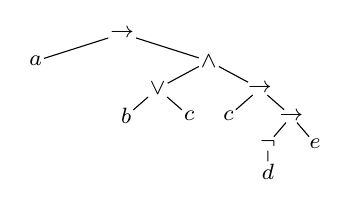
\begin{tikzpicture}[level distance=3.5mm,every node/.style={inner sep=0.6pt,font=\footnotesize},
level 1/.style={sibling distance=22mm},level 2/.style={sibling distance=13mm},level 3/.style={sibling distance=8mm},level 4/.style={sibling distance=6mm}]
\node{$\to$} child{node{$a$}} child{node{$\wedge$} child{node{$\vee$} child{node{$b$}} child{node{$c$}}} child{node{$\to$} child{node{$c$}} child{node{$\to$} child{node{$\neg$} child{node{$d$}}} child{node{$e$}}}}};
\end{tikzpicture}\par}
\sub{PL Q3: CNF}
\begin{itemize}
\item $\neg d\to e\equiv d\vee e$;\ $c\to(d\vee e)\equiv\neg c\vee d\vee e$; phân phối $\neg a$:
\item $F\equiv(\neg a\vee b\vee c)\wedge(\neg a\vee\neg c\vee d\vee e)=\gc{\gd{\neg a,b,c},\gd{\neg a,\neg c,d,e}}$.
\end{itemize}
\sub{FOL Q1--Q2}
\begin{itemize}
\item \textbf{Predicates} (toán hạng của $\to,\neg,\vee,\wedge$): $a$/2, $b$/3, $d$/1, $e$/1. \textbf{Functions} (nằm trong đối số): $c$/2 trong $b$, $f$/2 trong $e$, $g$/1 trong $f$.
\item Free: $\forall x.\exists y.$ chỉ buộc $x,y$ trong $(\neg b(\ldots)\vee d(x))$; $x,y$ trong $a(x,y)$, $e(\ldots)$ ở ngoài, $z$ không bao giờ bị lượng hóa: $\{x,y,z\}$.
\end{itemize}
\sub{Planning ($pX1_3$ = \texttt{posX-1-3}, $L2_3$ = \texttt{L-2-3})}
\begin{itemize}
\item Q1: $pX1_0\wedge\neg pX2_0\wedge\neg pX3_0\wedge pY1_0\wedge\neg pY2_0\wedge\neg pY3_0$. Q2 (5 bước): $pX2_5\wedge pY3_5$.
\item Q3 frame axioms posX lúc $t=3$ (2 / giá trị $\times$ 3 = 6):
\begin{itemize}
\item $(\neg pX1_3\wedge pX1_4)\to L2_3$;\ \ $(pX1_3\wedge\neg pX1_4)\to R1_3$
\item $(\neg pX2_3\wedge pX2_4)\to R1_3\vee L3_3$;\ \ $(pX2_3\wedge\neg pX2_4)\to R2_3\vee L2_3$
\item $(\neg pX3_3\wedge pX3_4)\to R2_3$;\ \ $(pX3_3\wedge\neg pX3_4)\to L3_3$
\end{itemize}
\item Q4 Up lúc $t=2$: $U1_2\to pY1_2\wedge\neg pY1_3\wedge pY2_3$; $U2_2\to pY2_2\wedge\neg pY2_3\wedge pY3_3$; $\neg U3_2$ (tiền điều kiện $Y<3$ sai).
\end{itemize}
\sub{Fuzzy}
\begin{itemize}
\item \textbf{Q1} $\frac{a+b}2$ \textbf{không} là T-norm: $T(.4,1)=.7\neq.4$.
\item \textbf{Q2} $R_{\min}(0.3,0.7)=1$ vì $0.3\le0.7$; $\vee$ = max: $\max(1,0.1)=\mathbf1$.
\item \textbf{Q3} Luật $c\ge\min(a,b)$, $a\ge c$; đầu $a=0,b=.3,c=.1$. Luật 2 nâng $a$ lên $.1$; ổn định: $\mathbf{a=.1,b=.3,c=.1}$.
\item \textbf{Q4} First of Maxima: $+$ luôn là điểm cực đại, đơn giản; $-$ bỏ qua cực đại khác (1960--2020 $\to$ 1960) và hình dạng.
\item \textbf{Q5} Không (trừ khi P = NP): quy SAT về (mục 10). \textbf{Q6} Có: PSL lồi, đa thức.
\item \textbf{Q7} $f=a+2\min(2-a-b,1)+3b$. Nếu $a+b\le1$: $f=a+2+3b$, tốt nhất trên $a+b=1$: $5-2a$. Nếu $a+b\ge1$: $f=4-a+b$. Max: $\mathbf{a=0,b=1}$, $f=5$.
\end{itemize}
\sub{FCA: ký hiệu; Q1}
\begin{itemize}
\item $x_1..x_7$ = Frodo, Aragorn, Gandalf, Legolas, Saruman, Boromir, Gollum; $y_1..y_7$ = Middle-earth, Warrior, Magic, Immortal, Ring-carrier, Fellowship, Evil.
\item \textbf{Q1 Có}: $x_2=x_6$ (gộp hàng); $y_1$ là cột đầy.
\item \textbf{Q2} hàng mới: $x_1{\cap}x_2=\{y_1y_6\}$, $x_1{\cap}x_5=\{y_1y_5\}$, $x_2{\cap}x_5=\{y_1\}$, $x_4{\cap}x_5=\{y_1y_4\}$, $x_3{\cap}x_5=\{y_1y_3y_4\}$; thêm $Y$ $\Rightarrow$ 12 intents (mọi intent chứa $y_1$):
\end{itemize}
\begin{minipage}[t]{0.6\linewidth}\vspace{0pt}
\setlength{\tabcolsep}{1.2pt}\renewcommand{\arraystretch}{0.92}
\begin{tabular}{@{}r|l|l|l@{}}
\# & intent & extent & dưới\\\hline
1 & $y_1$ & cả 7 & đỉnh\\
2 & $y_6$ & $x_1x_2x_3x_4x_6$ & 1\\
3 & $y_5$ & $x_1x_5x_7$ & 1\\
4 & $y_4$ & $x_3x_4x_5$ & 1\\
5 & $y_2y_6$ & $x_2x_3x_4x_6$ & 2\\
6 & $y_5y_6$ & $x_1$ & 2,3\\
7 & $y_5y_7$ & $x_5x_7$ & 3\\
8 & $y_3y_4$ & $x_3x_5$ & 4\\
9 & $y_2y_4y_6$ & $x_3x_4$ & 4,5\\
10 & $y_2y_3y_4y_6$ & $x_3$ & 8,9\\
11 & $y_3y_4y_5y_7$ & $x_5$ & 7,8\\
12 & $Y$ & $\emptyset$ & 6,10,11\\
\end{tabular}
\end{minipage}\hfill
\begin{minipage}[t]{0.39\linewidth}\vspace{4pt}
\centering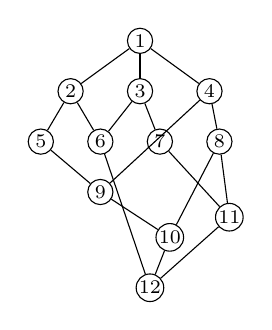
\begin{tikzpicture}[x=6.3mm,y=6.4mm,every node/.style={font=\scriptsize,inner sep=0.3pt}]
\foreach \n/\x/\y in {1/2/5,2/0.6/4,3/2/4,4/3.4/4,5/0/3,6/1.2/3,7/2.4/3,8/3.6/3,9/1.2/2,10/2.6/1.1,11/3.8/1.5,12/2.2/0.1}
  \node[circle,draw,minimum size=3.2mm] (c\n) at (\x,\y) {\n};
\foreach \a/\b in {1/2,1/3,1/4,2/5,2/6,3/6,3/7,4/8,4/9,5/9,9/10,8/10,8/11,7/11,6/12,10/12,11/12}
  \draw (c\a)--(c\b);
\end{tikzpicture}
\end{minipage}\par
\sub{FCA Q3--Q5}
\begin{itemize}
\item \textbf{Q3} ($\dn$ rồi $\up$): $y_6$: $\{x_1,x_2,x_3,x_4,x_6\}$, $\{y_1,y_6\}$: concept 2. $y_3$: $\{x_3,x_5\}$, $\{y_1,y_3,y_4\}$: 8. $y_2$: $\{x_2,x_3,x_4,x_6\}$, $\{y_1,y_2,y_6\}$: 5.
\item \textbf{Q4} $(\{x_3,x_5\},\{y_3,y_4\})$ \textbf{không}: $\{x_3,x_5\}\up=\{y_1,y_3,y_4\}$. $(\{x_1,x_2\},\{y_6\})$ \textbf{không}: $|\{y_6\}\dn|=5$.
\item \textbf{Q5} $\{y_2,y_6\}\to\{y_4\}$: $x_2,x_6$ không có $y_4$: \textbf{sai}; $s=\frac27$, $c=\frac24$. $\{y_5,y_6\}\to\{\neg y_7\}$: chỉ $x_1$, không có $y_7$: \textbf{đúng}; $s=\frac17$, $c=1$.
\end{itemize}
\sub{FCA Q6: luật kết hợp (AR) liên hệ với FCA thế nào}
\begin{itemize}
\item \kw{Cùng dữ liệu}: context = cơ sở dữ liệu transaction (đối tượng = transaction, thuộc tính = item); $\sigma(Z)=|Z\dn|$.
\item \kw{Liên hệ chính} \cnt{3}:
\begin{itemize}
\item \n1Implication $Z_1\Rightarrow Z_2$ = AR có confidence 100\%: $Z_1\dn\subseteq Z_2\dn\iff c=1$.
\item \n2Intents = \kw{closed itemsets}; $s(Z)=s(Z\dn{}\up)$, nên lattice lưu mọi support (iceberg lattice).
\item \n3Duquenne--Guigues = tập luật \emph{chính xác} ($c=1$) tối thiểu; AR thêm luật \emph{một phần} ($c<1$) trên minSup/minConf.
\end{itemize}
\item \kw{Dùng FCA}: dữ liệu nhỏ, sạch, cần luật \emph{luôn} đúng + phân cấp khái niệm (một hàng nhiễu phá implication).
\item \kw{Dùng AR}: dữ liệu lớn, nhiễu, luật đúng ``thường thường''; ngưỡng, thuật toán mở rộng được (Apriori, FP-Growth).
\item \kw{Ví dụ}: $\{y_2\}\Rightarrow\{y_6\}$: $s=\frac47$, $c=1$: implication và AR. $\{y_6\}\Rightarrow\{y_2\}$: $c=\frac45$ (Frodo $x_1$ là phản ví dụ): chỉ là AR.
\end{itemize}

\end{multicols*}
\end{document}
